\chapter{TINJAUAN PUSTAKA}
% Ubah konten-konten berikut sesuai dengan isi dari tinjauan pustaka
\section{Hasil penelitian terdahulu}
Penelitian mengenai identifikasi penyu pernah dilakukan oleh Christopher R. Gatto dengan judul penelitian “A novel method for photo-identification of sea turtles using scale patterns on the front flippers.” 
Penelitian tersebut dilakukan dengan mendeteksi keunikan visual dari sirip depan penyu dengan menggunakan "Automated Photo-Identification Suite" atau APHIS.
APHIS adalah alat yang didesain untuk mengidentifikasi individu hewan berdasarkan data fotografis.
APHIS memiliki kesulitan dalam melakukan identifikasi objek yang kompleks seperti pencahayaan atau latar yang berbeda.
Identifikasi yang digunakan pada penelitian tersebut menghasilkan akurasi sebesar 81.8\% untuk penyu dewasa. 
\parencite{GATTO201818}
Penelitian lain adalah artikel yang ditulis oleh Siti Nurfarahim Shaharudin berjudul "Comparison of Convolutional Neural Network Architectures for Sea Turtle Identification" mengeksplorasi penggunaan Convolutional Neural Network (CNN) untuk mengidentifikasi individu penyu.
Penelitian ini membandingkan arsitektur CNN berbeda, yaitu AlexNet dan GoogleNet.
Data yang dipakai adalah berbagai gambar individu penyu dengan memperhatikan fitur unik seperti pola pada cangkang, ukuran, bentuk, dan berbagai karakteristik fisik lainnya.
Pada arsitektur AlexNet, didapatkan akurasi sebesar 83.2\% dan presisi sebesar 82.1\%.
Sementara pada GoogleNet didapatkan akurasi sebesar 90.4\% dan presisi sebesar 88.2\%.
\parencite{10.1145/3616901.3617020}

\section{Dasar Teori}

\subsection{Vision Transformer}
Vision Transformer (ViT) adalah model deep learning berbasis transformer yang dirancang untuk mengolah data visual.
Model ini diperkenalkan oleh Dosovitskiy et al. (2020) papa artikel berjudul "An Image is Worth 16x16 Words: Transformers for Image Recognition at Scale" dan menjadi inovasi baru dalam bidang visi komputer karena mampu menyaingi CNN.
\parencite{dosovitskiy2021imageworth16x16words}
Model Transformer pada umumnya menerima  masukan berupa urutan \textit{token embedding} 1D.
Untuk mengolah data gambar 2D, gambar dibagi menjadi beberapa \textit{patch} 2D.
\textit{Patch} ini kemudian diubah menjadi representasi data vektor yang memiliki sifat yang sama dengan \textit{token} pada NLP.
Vektor \textit{patch} yang telah diratakan tersebut kemudian diproyeksikan secara linear ke dimensi yang lebih rendah, menghasilkan \textit{patch embedding} yang nantinya dapat menjadi masukan urut secara langsung ke model Transformer.
Karena model Transformer tidak memiliki cara untuk mengetahui posisi setiap \textit{patch embedding}, maka diperlukan tambahan \textit{positional embedding} berupa data 1D ke \textit{patch embedding}.
Seteleh mendapatkan deretan \textit{patch embedding} yang memiliki informasi posisi, kemudian akan diproses oleh \textit{encoder} pada standar model Transformer.
\textit{encoder} ini terdiri dari beberapa lapisan yang terdiri dari \textit{multihead self-attention} dan jaringan \textit{feed-forward}
jaringan \textit{self-attetntion} memungkinkan model untuk menangkap fitur dan hubungan lokal maupun global.
sebuah \textit{classification token} khusus sebelumnya ditanam pada deretan \textit{patch embedding}. 
Saat telah melalui \textit{encoder} dari transformer, keluaran yang sehubungan dengan \textit{token} tersebut akan menjadi representasi keseluruhan dari seluruh gambar.
representasi tersebut kemudian dimasukan ke MLP untuk menghasilkan klasifikasi akhir.
\parencite{dosovitskiy2021imageworth16x16words}

\begin{figure} [H] \centering
  % Nama dari file gambar yang diinputkan
  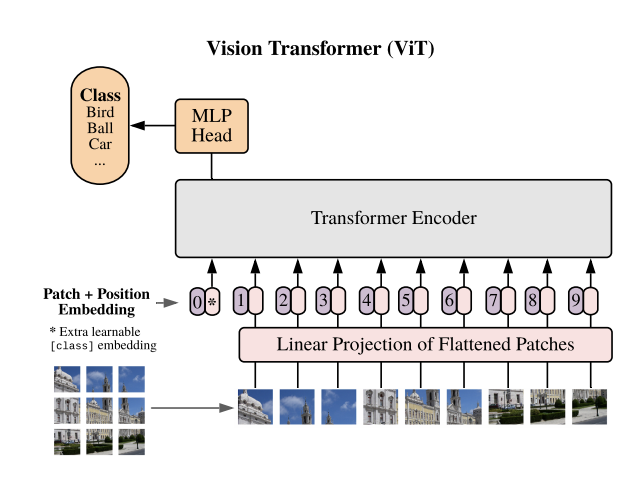
\includegraphics[scale=0.45]{gambar/ViTSchema.png}
  % Keterangan gambar yang diinputkan
  \caption{ skema cara kerja Vision Transformer \parencite{dosovitskiy2021imageworth16x16words}}
  % Label referensi dari gambar yang diinputkan
  \label{fig:ViTSchema}
\end{figure}

Saat dilakukan \textit{training} dengan dataset JFT-300M yang memiliki 300 juta gambar dengan label, didapatkan akurasi sebesar 88\% yang lebih dari model CNN seperti ResNet-152 yang memiliki akurasi sebesar 83.3\% pada dataset yang sama dan EfficientNet yang memiliki akurasi sebesar 83-85\% pada dataset yang sama.
Saat dilakukan \textit{training} dengan dataset yang lebih kecil seperti ImageNet-21k yang memiliki 14 juta gambar dengan label, didapatkan akurasi yang lebih kecil dikarenakan sifat ViT yang sangat membutuhkan data dengan jumlah besar.
\parencite{dosovitskiy2021imageworth16x16words}

\subsection{Vision Transformer untuk Re-Identifikasi}
Re-Identifikasi (Re-ID) adalah proses penyocokan visual individu atau objek di berbagai kondisi berbeda.
Model Re-ID dapat digunakan pada berbagai kamera yang berbeda dengan sudut penangkapan gambar yang berbeda juga.
Selain itu, keunggulan Re-ID dengan identifikasi biasa adalah Re-ID dapat melakukan identifikasi dengan perbedaan pencahayaan dan latar yang berbeda.
\parencite{zheng2016person}

Terciptanya Vision Transformer (ViT) memiliki pengaruh terhadap perkembangan dalam teknologi Re-ID.
Dengan berkembangnya ViT, Re-ID yang sebelumnya secara umum dilakukan dengan menggunakan CNN, kini mengalami peningkatan performa yang signifikan.
Perkembangan ini dapat terlihat dengan adanya keunggulan pada skalabilitas dan fleksibilitas model Re-ID yang memanfaatkan mekanisme textit(attention) yang dimiliki oleh model berbasis Transformer.
Pada artikel berjudul "Transformer for Object Re-Identification: A Survey" yang ditulis oleh Mang Ye, dijelaskan bagaimana meningkatnya performa penggunaan model Transformer dibandingkan dengan penggunaan model CNN.
Artikel ini juga memberikan model Transformer baru yang yang didesain untuk aplikasi Re-ID yang bernama UntransReID.
UntransReID memberikan performa yang dapat mengungguli model-model terbaru dengan akurasi sebesar 96.7\% pada Market-1501 dataset dan akurasi sebesar 87.5\% pada MSMT17 dataset.
\parencite{ye2024transformerobjectreidentificationsurvey}
\begin{figure} [H] \centering
  % Nama dari file gambar yang diinputkan
  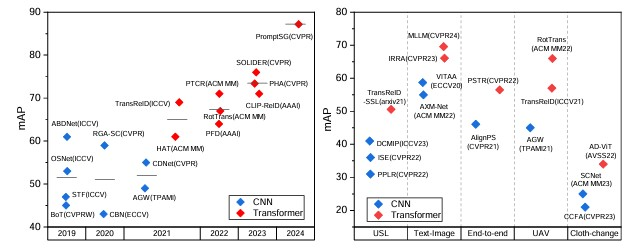
\includegraphics[scale=0.45]{gambar/ViT-ReID.jpg}
  % Keterangan gambar yang diinputkan
  \caption{Grafik Performa Transformer dibandingkan CNN \parencite{ye2024transformerobjectreidentificationsurvey}}
  % Label referensi dari gambar yang diinputkan
  \label{fig:ViTPerformance}
\end{figure}

\subsection{Ekstraksi Pola Kepala Penyu}
Penyu memmiliki pola sisik kepala yang unik dan berbeda pada setiap individu.
Selain itu terdapat perbedaan pola pada setiap spesies penyu.
Pola, peletakan, dan bentuk spesifik pada penyu sisik akan selalu sama dan konsisten pada setiap individu, memungkinkan identifikasi dan pembedaan pada setiap individu penyu dengan spesies yang sama.
\parencite{ecomarBelizeAnatomy}

Pada penelitian berjudul "Enhancing sea turtle photo identification: a comparative analysis of a self-developed noninvasive automated algorithm versus the manual HotSpotter method" yang ditulis oleh A. Rios-Ramos, menjelaskan pendekatan berbasis kecerdasan buatan (AI) untuk mengidentifikasi individu penyu menggunakan \textit{Photo Identification} (Photo-ID).
Metode ini melibatkan deteksi otomatis dengan menggunakan pola pada kepala penyu menggunakan YOLOv5.
\parencite{10.1117/12.3028422}
Kontribusi signifikan dalam ekstraksi pola kepala penyu adalah "SeaTurtleID2022: A long-span dataset for reliable sea turtle re-identification" yang memberikan dataset sejumlah 8,729 foto dari 438 individu unik yang diambil selama lebih dari 13 tahun.
\parencite{adam2024seaturtleid2022longspandatasetreliable}
Extraksi dan analisa pola unik pada penyu adalah faktor krusial untuk melakukan identifikasi individu.